\documentclass{standalone}
\usepackage{tikz}
\begin{document}
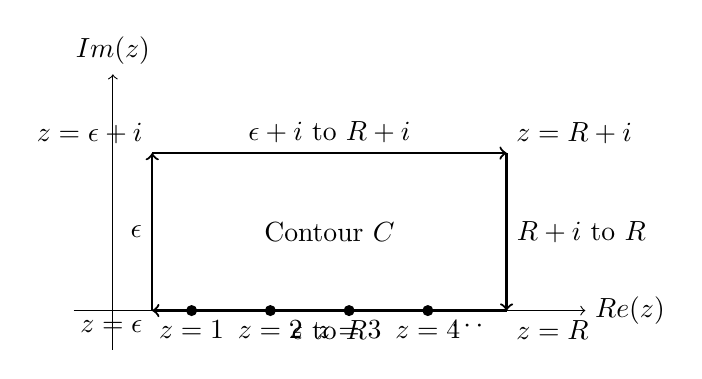
\begin{tikzpicture}
% Axes
\draw[->] (-0.5,0) -- (6,0) node[right] {$\text{Re}(z)$};
\draw[->] (0,-0.5) -- (0,3) node[above] {$\text{Im}(z)$};

% Contour path (counterclockwise)
\draw[thick,->] (5,0) -- (0.5,0) node[midway,below] {$\epsilon$ to $R$};
\draw[thick,->] (0.5,0) -- (0.5,2) node[midway,left] {$\epsilon$};
\draw[thick,->] (0.5,2) -- (5,2) node[midway,above] {$\epsilon + i$ to $R + i$};
\draw[thick,->] (5,2) -- (5,0) node[midway,right] {$R + i$ to $R$};

% Poles along real axis
\foreach \x in {1,2,3,4} {
  \fill (\x,0) circle (2pt);
  \node[below] at (\x,0) {$z = \x$};
}
\node[below] at (4.5,0) {$\cdots$};

% Labels for vertices
\node[below left] at (0.5,0) {$z = \epsilon$};
\node[above left] at (0.5,2) {$z = \epsilon + i$};
\node[above right] at (5,2) {$z = R + i$};
\node[below right] at (5,0) {$z = R$};

% Annotation for contour direction
\node at (2.75,1) {Contour $C$};
\end{tikzpicture}
\end{document}